\section{Durchführung}
\label{sec:Durchführung}


\subsection{Bestimmung der Kennlinien}
\label{sec:Kennlinien}

\begin{figure}
    \centering
    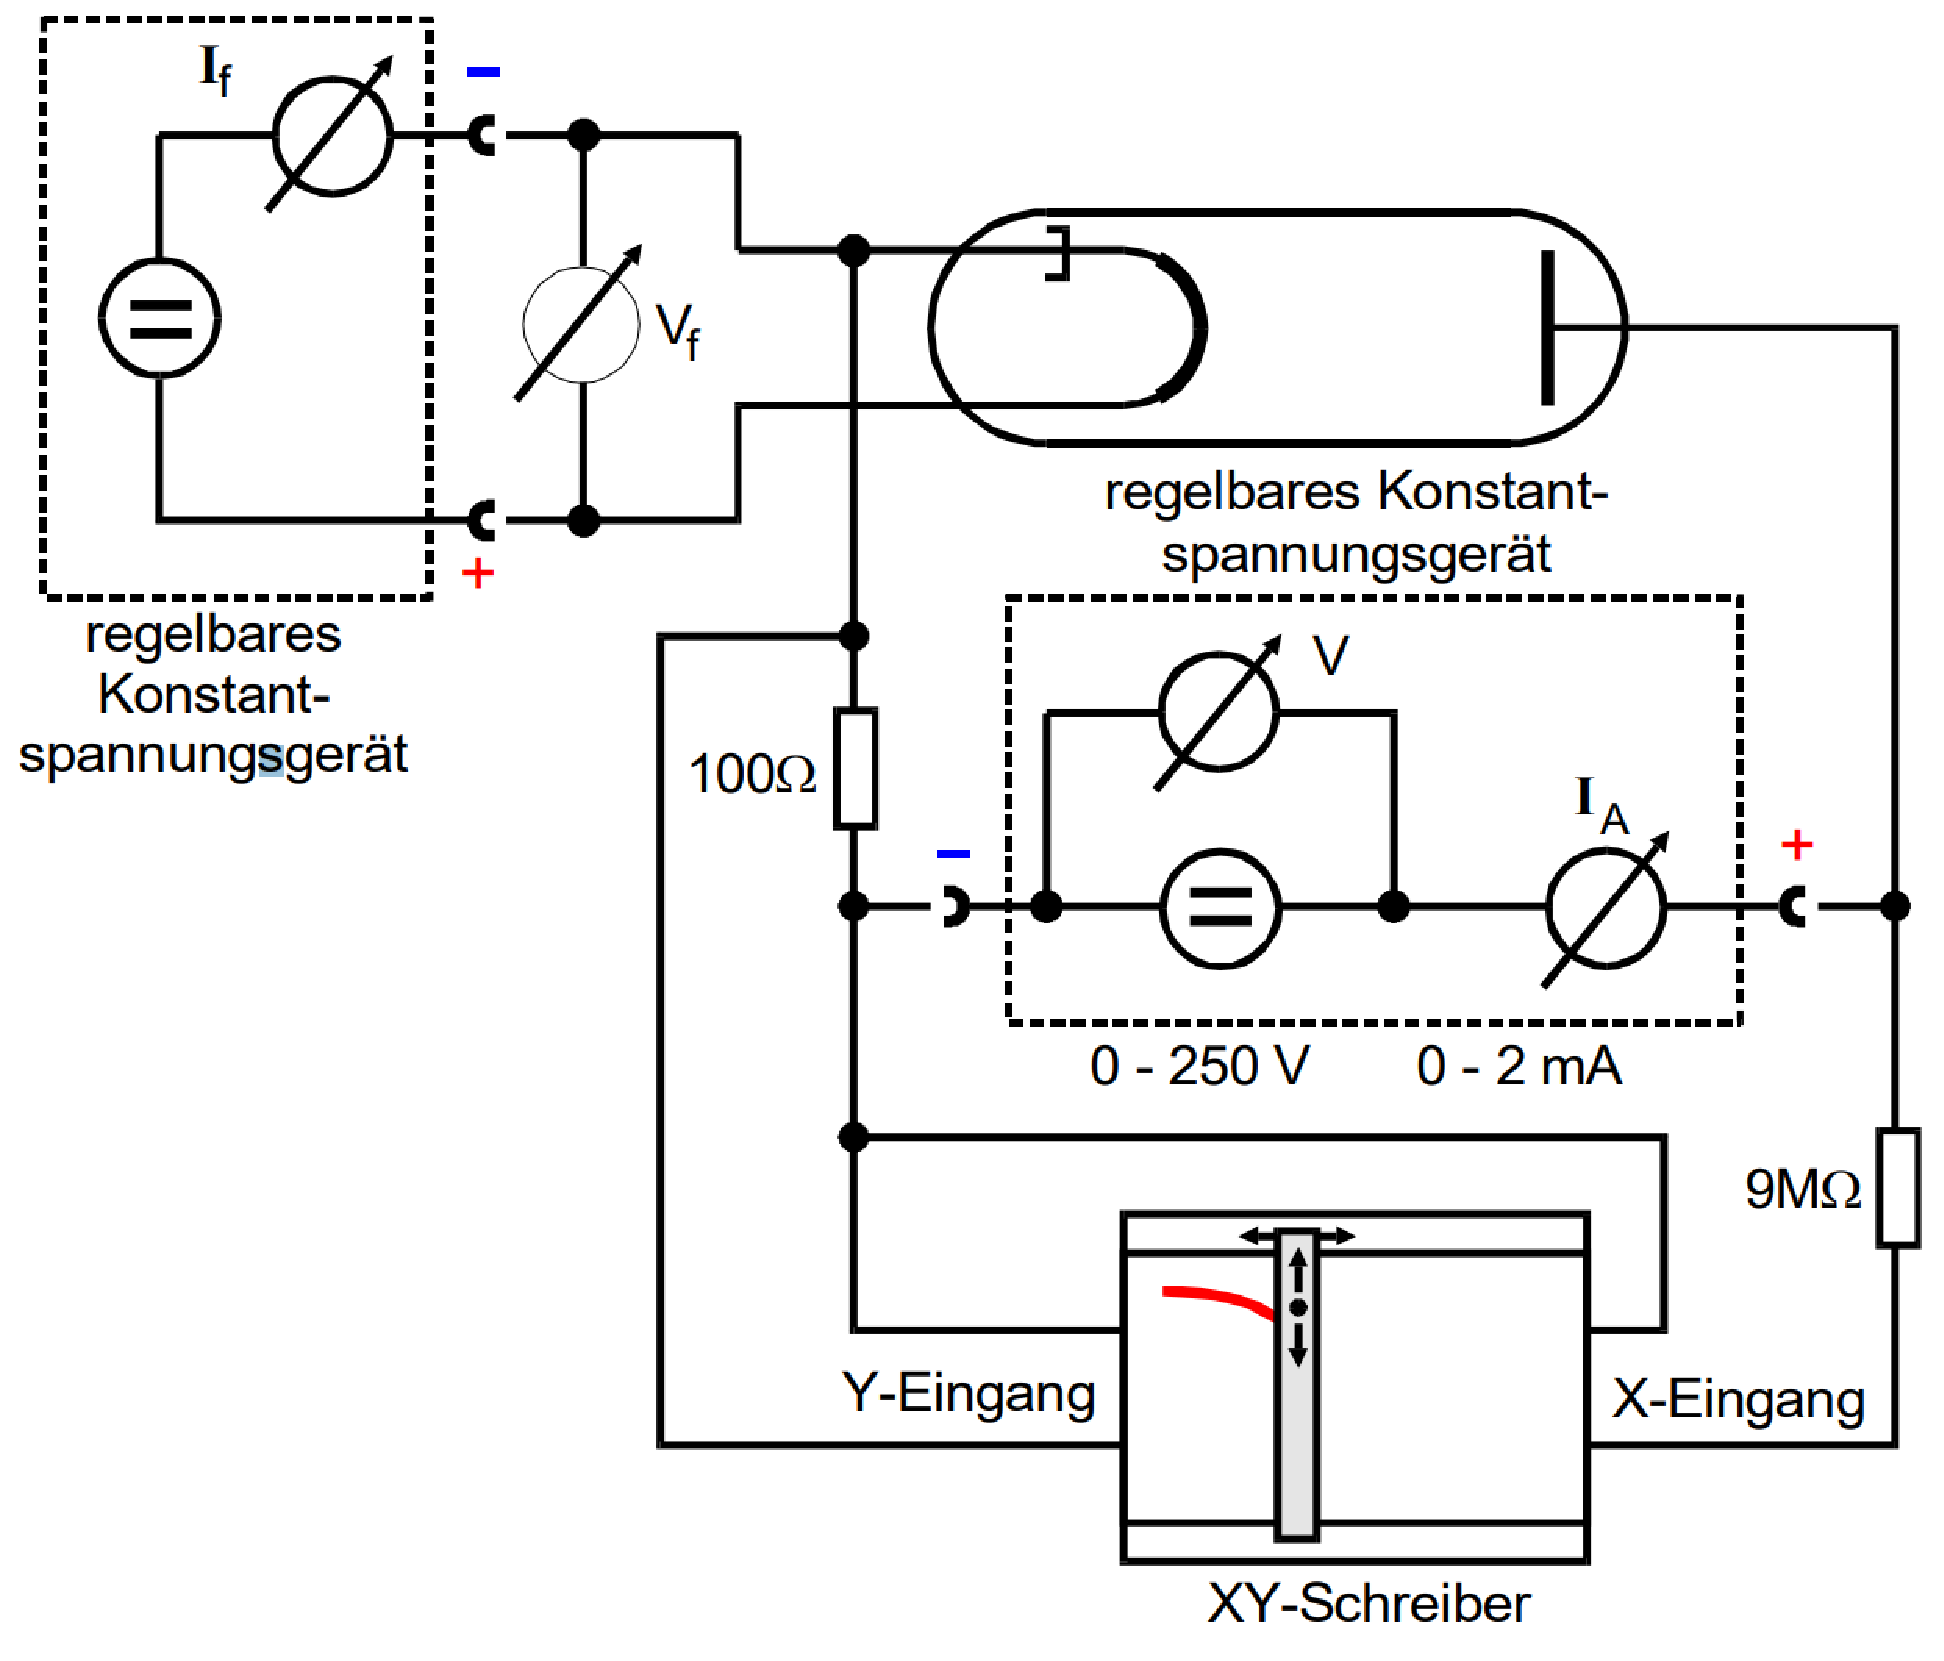
\includegraphics[width=0.7\textwidth]{pictures/Aufbau.pdf}
    \caption{Schaltung zur Aufnahme von Diodenkennlinien \cite{v504}.}
    \label{fig:Aufbau}
\end{figure}

Der genaue Versuchsaufbau wird in \hyperref[fig:Aufbau]{Abbildung \ref{fig:Aufbau}} dargestellt.
Im Aufbau im Labor wird der untere Teil durch ein einzelnes Bauteil zusammengefasst.
Die Kathode der Diode wird dann durch den Heizstrom erwärmt, wodurch diese dann die Elektronen emittiert.
Diese werden dann durch die Anodenspannung $U_A$ zur Anode hin beschleunigt.
Die Heizspannung wird maximal eingestellt und der Heizstrom wird auf $1,9 \unit\ampere$ gestellt.
Die Anodenspannung (Beschleunigungsspannung) wird dann von $0 \unit\volt$ auf $250 \unit\volt$ in Schritten hochgestellt.
Dabei wird dann der Strom an der Anode abgelesen und notiert.
Diese Messung wird für verschiedene Heizströme zwischen $1,9 \unit\ampere$ und $2,4 \unit\ampere$ durchgeführt

\subsection{Aufnahme der Anlaufstromkurve}

\begin{figure}
    \centering
    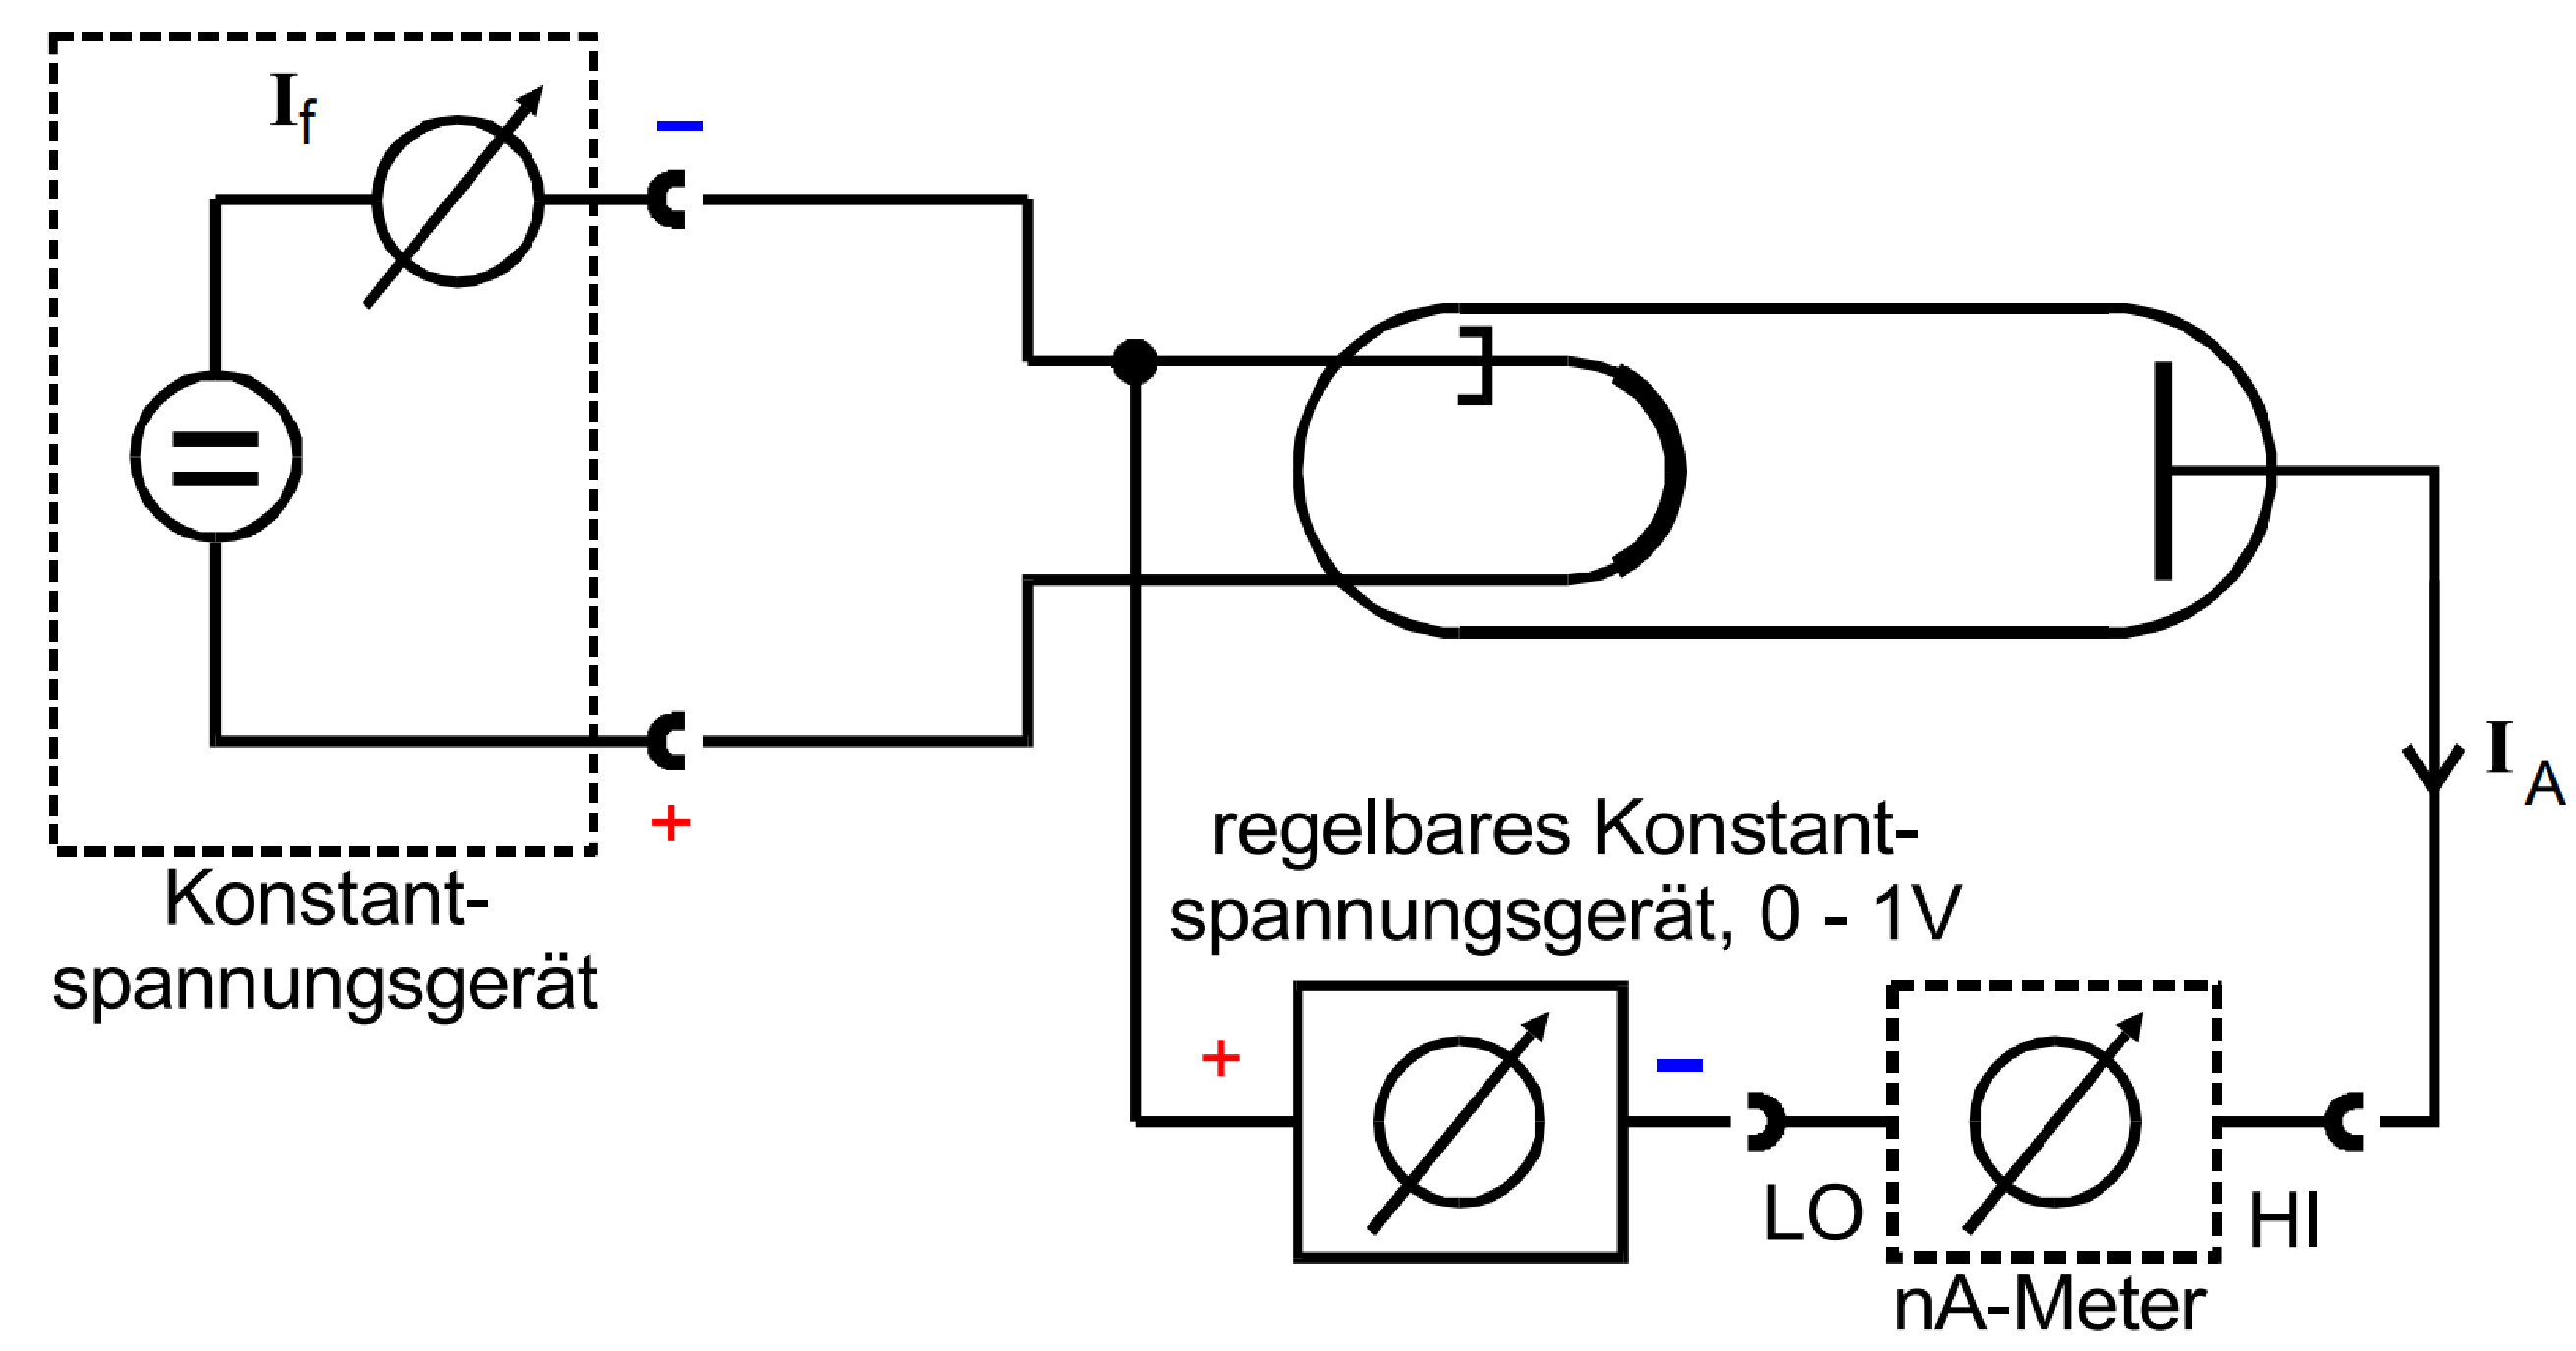
\includegraphics[width=0.7\textwidth]{pictures/Aufbau2.pdf}
    \caption{Schaltung zur Aufnahme einer Anlaufstromkurve \cite{v504}.}
    \label{fig:Aufbau2}
\end{figure}

Für diese Messung wird die Schaltung in \hyperref[fig:Aufbau2]{Abbildung \ref{fig:Aufbau2}} nachgebildet.
Es wird ein Heizstrom von $2,4 \unit\ampere$ eingestellt und die Heizspannung wird maximal eingestellt.
Die Gegenspannung wird nun von $0 \unit\volt$ bis $ 1 \unit\volt$ in Schritten hochgestellt
und der absinkende Stromfluss wird am Messgerät wird abgelesen und notiert.